\documentclass[12pt]{article}
\usepackage[utf8]{inputenc}
\usepackage[english, russian]{babel}
\usepackage{amsmath,amsfonts,amssymb,euscript,graphicx,wrapfig,multirow}
\usepackage{dsfont}
\usepackage{amsthm}
\usepackage{textcomp}
\textheight=240mm \textwidth=170mm
\hoffset=-17mm % сдвиг влево
\voffset=-17mm % сдвиг вверх

\usepackage{hyperref}

\begin{document}

\selectlanguage{russian}

\noindent УДК~519.146

\begin{center}
\textbf{О некоторых оценках диаметра целоудалённых множеств точек в многомерных пространствах} \\[3mm]
\textbf{Р.~Е.~Зволинский, Е.~А.~Момот} \\[2mm]
\emph{ВГУ}
\end{center}

\section{Введение}

Настоящая работа имеет целью кратко изложить (на русском языке) содержание работы [1], дополнив его некоторыми результатами
вычислений и подробностями используемых алгоритмов.

\par
\textbf{Определение 1.}
Целоудалённым множеством $\mathcal{P}$ называют множество точек в
$m$-мерном евклидовом пространстве $\mathbb{R}^{m}$, такое, что расстояние
между любыми двумя точками этого множества есть целое число.

Если $m = 2$, то такое ЦМ будем называть \textit{плоским}.

Как можно охарактеризовать целоудалённое множество?
Во-первых, мы можем подсчитать количество точек в нём,
которое всегда конечно [2, 3], далее будем называть это число \textit{мощностью};
во-вторых, мы можем естественным образом определить диаметр конечного множества точек.

\par
\textbf{Определение 2.}
Диаметр конечного множества $\mathcal{P}$ определяется как
\begin{equation}
\operatorname{diam(\mathcal{P})} = \underset{P_{1}, P_{2} \in
\mathcal{P}}{\max} |P_{1}P_{2}|,
\end{equation}
где $|P_1 P_2|$ есть обычное расстояние между точками.

У каждого ЦМ также есть характеристика
[4, 5].

\par
\textbf{Определение 3.}
Функция $d(m, n)$ есть минимальный возможный диаметр ЦМ $\mathcal{P}$ мощности $n$
в $m$-мерном евклидовом пространстве $\mathbb{R}^{m}$.

Список известных оценок функции $d(m, n)$
читатель может найти в [6, Theorem 1] или в [7].
Кроме того, определённый прогресс был достигнут в работе [8]. %Nozaki 2018
Мы обсудим следующие оценки, представленные в [6]:
\begin{align}
	&d(m, 2m + 1) \leq 8 \\
	&d(m, 2m + 2) \leq 13 \\
	&d(m, 3m) \leq 109
\end{align}
и следующую теорему [6, Theorem 2.1].

\par
\textbf{Теорема 1.}
Пусть $\mathcal{P}$ -- плоское целоудалённое множество точек,
где $(n - 2)$ точки  расположены на прямой $l_{1}$, а две точки
$P_{1}$ и  $P_{2}$ на параллельной ей прямой $l_{2}$, при этом расстояние
между $l_{1}$ и $l_{2}$ равно $r$. Если существуют положительные целые числа
$v$, $w$, удовлетворяющие условиям $f^{2} + v^{2}
= w^{2}$ и $v < 2r$, где $|P_{1}P_{2}| = f$,
то

\begin{equation}
d(m, n - 2 + 2(m - 2)) \leq \max(w, \operatorname{diam(\mathcal{P})})
.
\end{equation}

В данной статье мы представим некоторые оценки функции $d(m,n)$, основанные на плоских ЦМ определённых типов.

\section{Классификация ЦМ, расположенных на двух прямых}


Терминология, сложившаяся при классификации ЦМ под влиянием С. Курца, весьма своеобразна. Он использовал такие наименования, как
<<crab>> и даже <<semi-crab>> [9]. %TODO:Antonov, Kurz
При переводе этой терминологии мы будем использовать прилагательные, следуя [7]. %TODO:обзорник

\par
\textbf{Определение 4.}
Плоские целоудалённые множества мощности $n$, для которых можно найти такую прямую $l_1$, что
$(n - 1)$ точек лежит на $l_1$, будем называть \textit{веерными}.

\par
\textbf{Определение 5.}
Плоские целоудалённые множества мощности $n$, для которых можно единственным образом найти такие прямые $l_1$, $l_2$,
что $k$ точек лежат на прямой $l_1$, а $(n - k)$ -- на прямой $l_2$, причём $k \geq 2$, будем называть \textit{рельсовыми}.

Среди рельсовых систем наиболее распространены ЦМ с двумя точками на одной прямой и остальными на другой.

\par
\textbf{Определение 6.}
\textit{Ножничными} будем называть такие плоские целоудалённые множества мощности $n$, для которых можно единственным
образом найти такие прямые $l_1$, $l_2$, что $k$ точек лежат на прямой $l_1$, а $(n - k)$ -- на прямой $l_2$, причём $k \geq 2$ и
прямые $l_1$ и $l_2$ не являются ни параллельными, ни перпендикулярными.

Существует важный подкласс ножничных систем.

\par
\textbf{Определение 7.}
Ножничные системы с осью симметрии,
являющейся биссектрисой угла между прямыми, назовём \textit{пирамидальными}.

\par
\textbf{Определение 8.}
\textit{Крестовыми} будем называть такие плоские целоудалённые множества мощности $n$, для которых можно единственным
образом найти такие прямые $l_1$, $l_2$, что $k$ точек лежат на прямой $l_1$, а $(n - k)$ -- на прямой $l_2$, причём $k \geq 2$ и
$l_1$ перпендикулярна $l_2$.

\section{Оценки, основанные на рельсовых системах}

Пусть $i = \overline{1, k}$ обозначает перечисление всех $i$
от $1$ до $k$.
Теорему [6, Theorem 2.1] можно обобщить
следующим образом:

\par
\textbf{Теорема 2.}
Пусть $\mathcal{P}$ -- плоское целоудалённое множество точек, где
$k$ точек $P_1$, $P_2$, $\ldots$, $P_k$ последовательно расположены на
прямой $l_1$, а $(n - k)$ точек -- на параллельной ей прямой $l_2$,
при этом расстояние между $l_1$ и $l_2$ равно $r$.
Если существуют положительные целые числа $v$, $w_{ij}$, удовлетворяющие
условиям $f_{ij}^{2} + v^{2} = w_{ij}^{2}$ и $v < 2r$, где
$i = \overline{1, k - 1}$, $j = \overline{i + 1, k}$, $|P_{i}P_{j}| = f_{ij}$,
то

\begin{equation}
d(m, n + k(m - 2)) \leq \max(w_{1k}, \operatorname{diam(\mathcal{P})})
.
\end{equation}

Ниже мы приводим оценки функции $d(m, n)$ для $n = 2m + k$, $3 \leq k \leq 24$, а также для $n = 4m$, основанные на рельсовых ЦМ (подробное описание данных ЦМ и конструкций для построения оценок можно найти в [1]).
\begin{align*}
&(d(m, 2m + k))_{k = 3, \ldots, 24} \leq 158,\, 158,\, 252,\, 297,\, 1073,\, 1273,\, 1888,\, 2189,\, 3224,\, 3696,\, 5141,\, 6586,\, \\
&11692,\, 12296,\, 16027,\, 19758,\, 32054,\, 39516,\, 254364,\, 276612,\, 338169,\, 399726
\end{align*}

Р. Гай в своей работе [10, D 20] приводит ЦМ из $8$ точек, расположенное на двух параллельных прямых. С помощью теоремы 2 можно построить следующую оценку:
\begin{equation}
d(m, 4m) \leq 409
\end{equation}

Также с помощью ЭВМ нам удалось получить рельсовую ЦМ мощности 40 (на данный момент это наибольшая по мощности рельсовая ЦМ, которую нам удалось найти).

Для облегчения восприятия применяется запись вида
[7, 11, 12]:
$\sqrt{p}/q * \{ (x_1,y_1), \ldots,$ $ (x_n, y_n)  \}$,
означающая, что каждую абсциссу нужно умножить на $1/q$,
а каждую ординату -- на $\sqrt{p}/q$, т.е.
\begin{align} \label{notation}
	\sqrt{p}/q * \{ (x_1,y_1), ..., (x_n, y_n)  \}
	=
	\left\{ \left(\frac{x_1}{q},\frac{y_1\sqrt{p}}{q}\right), ..., \left(\frac{x_n}{q},   \frac{y_n\sqrt{p}}{q}\right)  \right\}.
\end{align}

\begin{figure}[h!]
	\begin{center}
	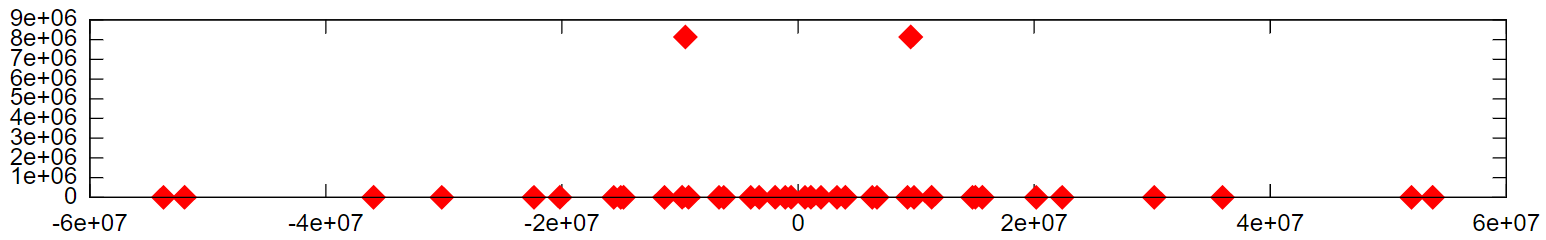
\includegraphics[width=1.1\linewidth]{picture_40.png}
	\parbox{1\linewidth}{\caption{ЦМ мощности 40, диаметр 107526848}
	\label{picture_40.png}}
	\end{center}
\end{figure}

\begin{itemize}
\setlength{\itemsep}{-1mm}

\item
$\mathcal{P}=\sqrt{154}/{1} * \{ (\pm 53763424, 0),
(\pm 51964380 , 0),
(\pm 35959560 , 0),
(\pm 30175080 , 0),
(\pm 22378720 , 0),
$

$
(\pm 20180160 , 0),
(\pm 15613780 , 0),
(\pm 15025920 , 0),
(\pm 14779380 , 0),
(\pm 11313120 , 0),
(\pm 9817080 , 0),
$

$
(\pm 9544080 , 655200),
(\pm 9271080 , 0),
(\pm 6693960 , 0),
(\pm 6289920 , 0),
(\pm 4006275 , 0),
(\pm 3290560 , 0),
$

$
(\pm 1938720 , 0),
(\pm 1092000 , 0),
(\pm 583648 , 0)\}
$
(Рис.~\ref{picture_40.png}).

$f = 19088160$, $v = 8738$, $w = 19088162$, $\operatorname{diam(\mathcal{P})}
= 107526848$,

что даёт оценку $d(m, 2m + 34) \leq 107526848$.

\end{itemize}


\section{Оценки, основанные на пирамидальных системах}

\par
\textbf{Теорема 3.}
Пусть $\mathcal{P}$ -- плоское целоудалённое множество точек, где
$k$ точек расположены на прямой $l_{1}$ и $k$ точек на прямой $l_{2}$.
Пусть, кроме того, эти точки симметричны относительно одной из биссектрис углов пересечения
прямых $l_{1}$ и $l_{2}$, тогда

\begin{equation}
d(m, (k - \alpha)m + \alpha) \leq \operatorname{diam(\mathcal{P})},
\end{equation}

где
\begin{equation*}
\alpha =
\begin{cases}
1, \text{если точка пересечения} \in \mathcal{P}, \\
0, \text{если точка пересечения} \notin \mathcal{P}.
\end{cases}
\end{equation*}

\par
\textbf{Замечание 1.}
Углы могут быть острыми или тупыми, но, очевидно, не прямыми [1, Remark 2].

Ниже мы приводим оценки функции $d(m, n)$ для $n = 3m + 1$ и $n = 4m + 1$, основанные на пирамидальных ЦМ (подробное описание данных ЦМ и конструкций для построения оценок можно найти в [1]).

\begin{align}
&d(m, 3m + 1) \leq 56 \\
&d(m, 4m + 1) \leq 1260
\end{align}

Получившаяся оценка для функции $d(m, 3m + 1)$ улучшает оценку для $d(m, 3m)$, представленную в [4].

\section{Особенности алгоритмов}
Используется алгоритм, описанный в [13], со следующими модификациями:

Во-первых, изначальный граф разбивается на несколько подграфов в зависимости от характеристик. Треугольники, образованные вершинами каждого подграфа, имеют одинаковую характеристику, т.е. каждому подграфу сооветствует своя
характеристика.

Во-вторых, мы стараемся как можно раньше исключать точки, входящие только в веерные системы, поскольку веерные системы
нам не интересны.

В-третьих, используется длинная целая арифметика и новый тип BigInt языка Javascript.

За представление ЦМ отвечает класс PointSet, следующий представлению (\ref{notation}), что позволяет оперировать только с целыми числами.
В дальнейшем операции проводятся лишь над точками, имеющими совместное представление (\ref{notation}).

Основной классификационный инструмент -- это функция, находящая все точки заданного множества, не лежащие на прямой, проходящей через две заданные точки.

Реализованы и другие необходимые иструменты, такие как проверка прямых на параллельность в условиях представления каждой прямой парой точек
с координатами вида (\ref{notation}), а также прочие проверки, позволяющие классифицировать ЦМ в терминах [9]
(например, отыскивать центр окружности по заданным трём точкам в соответствующем представлении через целые числа).
Большая часть функций покрыта юнит-тестами с использованием библиотек ‘chai’ и
<<мокко>>.
%(TODO: списать из отчёта).

Следуя идеологии NodeJS/NPM, часть переиспользуемого кода выделена в библиотеки
‘json-bigint-native’ (см. https://www.npmjs.com/package/bigint-json-native), ‘bigint-isqrt’ (см. https://www.npmjs.com/package/bigint-isqrt)
и ‘bigint-is-perfect-square’ (см.

\noindent https://www.npmjs.com/package/bigint-is-perfect-square).
 %(TODO: списать, какие, + ссылки как на электронные ресурсы).

Визуализация найденных множеств производится с помощью gnuplot [14].


\section{Заключительные замечания}

Все данные ЦМ были получены путём сочетания компьютерного перебора и интуиции авторов;
таким образом, дальнейший поиск может привести к лучшим оценкам, использующим ту же
конструкцию.

До сих нет общей конструкции для рельсовых или ножничных систем заданной мощности.

Для рельсовых ЦМ мы можем предположить, что существует множество произвольной мощности с $2$ точками на одной линии, а все остальные на другой; с другой стороны,
мы до сих пор не нашли ни одной рельсовой ЦМ с $4$ и $5$ точками на <<отделившихся>> прямых.

На сегодняшний день мы нашли пирамидальные ЦМ мощности не более $9$.

Исходный код можно получить по адресам https://gitlab.com/Nickkolok/ips-algo,

https://gitlab.com/Aisse-258/ips-algo.

\bigskip\centerline{\bf Литература}

1.  \emph{ Avdeev N.~N., Zvolinsky R.~E., Momot E.~A.} On particular diameter bounds
for integral point sets in higher dimensions. -- 2019. -- arXiv: 1909.10386v1

2.	\emph{ Anning N.~H., Erd{\"o}s P.} Integral distances // Bulletin of the American Mathematical Society. -- 1945. -- Vol. 51, no. 8. -- Pp. 598-600. -- DOI: 10.1090/S0002-9904-1945-08407-9.

3.	\emph{ Erd{\"o}s P.} Integral distances // Bulletin of the American Mathematical Society. -- 1945. -- Vol. 51, no. 12. -- P. 996. -- DOI: 10.1090/S0002-9904-1945-08490-0.

4.  \emph{ Kemnitz A.} Punktmengen mit ganzzahligen Abst{\"a}nden. -- 1988.

5.  \emph{ Kurz S.} On the characteristic of integral point sets in $\mathbb{E}^m$ // Australasian Journal of Combinatorics. -- 2006. -- Vol.~36. -- Pp. 241-248. --
arXiv: math/0511704.

6.  \emph{ Kurz S., Laue R.} Bounds for the minimum diameter of integral point sets
// Australasian Journal of Combinatorics. -- 2007. -- Vol.~39. -- Pp. 233-240. --
arXiv: 0804.1296.

7.  \emph{ Авдеев Н.~Н., Семёнов Е.~М.} Множества точек с целочисленными расстояниями на плоскости и в евклидовом пространстве // Математический форум
(Итоги науки. Юг России). -- 2018. -- Pp. 217-236.

8.  \emph{ Nozaki H.} Lower bounds for the minimum diameter of integral point sets
// Australasian Journal of Combinatorics. -- 2013. -- Т.~56. -- С. 139-143.

9.  \emph{ Antonov A.~R., Kurz S.} Maximal integral point sets over
$\mathbb{Z}^{2}$ // International Journal of Computer Mathematics. -- 2008. --
Vol.~87, no.~12 -- Pp. 2653-2676. -- DOI:

\noindent 10.1080/00207160902993636. -- arXiv: 0804.1280.

10.  \emph{ Guy R.} Unsolved problems in number theory. Vol. 1. -- Springer Science \& Business Media, 2013. -- DOI: 10.1007/978-1-4757-1738-9.

11.  \emph{ Авдеев Н.~Н.} On integral point sets in special position // Некоторые вопросы анализа, алгебры, геометрии и математического образования: материалы международной молодежной научной школы <<Актуальные направления математического анализа и смежные вопросы>>. -- 2018. -- Vol.~8. -- Pp. 5-6.

12.  \emph{ Авдеев Н.~Н.} Об отыскании целоудалённых множеств специального вида
// Актуальные проблемы прикладной математики, информатики и механики --
сборник трудов Международной научной конференции. -- Научно-исследовательские публикации, 2018. -- Pp. 492-498.

13.  \emph{ Авдеев Н.~Н.} Об отыскании множеств точек на плоскости с целочисленными
расстояниями // Математическое и компьютерное моделирование, информационные технологии управления: сб. тр. Школы для студентов, аспирантов и молодых учёных
<<МКМИТУ-2016>>. -- 2016. -- С. 15-19.

14.  \emph{ Балдин Е.} Графики заказывали? // Системный администратор. -- 2007. --
\textnumero.~4. -- С. 72-77.


{\bf Зволинский Роман Евгеньевич},
студент кафедры теории функций и геометрии математического факультета ФГБОУ ВО <<Воронежский государственный университет>>, г. Воронеж.

E-mail: roman-zvolinskiy@mail.ru

Научный руководитель: Семенов Евгений Михайлович.

{\bf Момот Екатерина Александровна},
студент кафедры функционального анализа и операторных уравнений математического факультета
ФГБОУ ВО <<Воронежский государственный университет>>, г. Воронеж.

\end{document}







